\documentclass[12pt]{article}
\usepackage{graphicx}
\usepackage{gensymb}

\begin{document}
\graphicspath{ {images/} }
\section*{About Network Training}

The network training part on the second tab \textit{Network Training} is initially not activated, until you select datasets. 

\subsection{Select datasets}
Click the button \textit{Select Database}, you can select the path into a desired database, then the path will be shown after the button, and the patients and sequences will be shown separately in two lists. Then, you can check on patients and sequences. When both are selected, a \textit{Datasets Window} will pop up and showing the combination of image paths you selected, if you do not want to select training/validation/test datasets manually, just ignore it (or close it). When you want to split the datasets by yourself, please remember to select all three groups of training/validation/test in the drop down box on the right side of each dataset path, only when all three groups are selected, the splitting mode can be set as self-defined. Finally, please click on any image item to confirm the changes. 
\begin{figure}[htbp]	
	\centering
	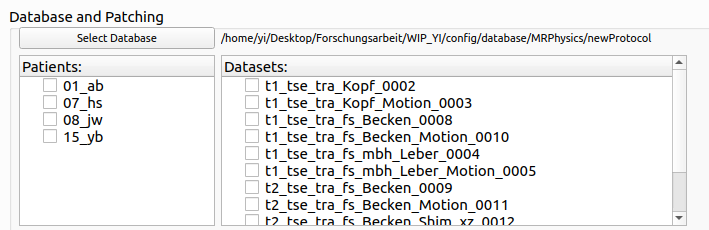
\includegraphics[width=\textwidth]{select_datasets.png}
	\caption[Select Datasets]{Select Datasets}
	\label{fig:select_datasets}
\end{figure}
\begin{figure}[htbp]	
	\centering
	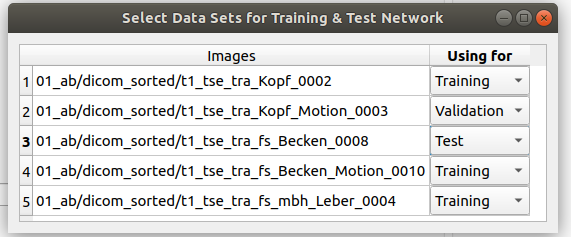
\includegraphics[width=\textwidth]{datasets_interface.png}
	\caption[Datasets Interface]{Datasets Interface}
	\label{fig:datasets_interface}
\end{figure}

\subsection{Patching images}
There are several options for generating datasets by patching. At first, you should set the \textit{Output Path} correctly, where you want to save the datasets. Then, you can select 2D/3D patching with matching patch sizes to the neural network you want to train later on. If you select 2D patching, the third patch size will be ignored. And If you select the labeling mode as mask labeling or 2D patch labeling, you should also set a suitable overlap. Besides, you can select the methods of sample splitting mode, if you do not split datasets by yourself. There are three methods provided, simple random sample splitting, cross validation splitting and patient cross validation splitting. For simple random sample splitting, the training/validation/test datasets will be split by corresponding ratio, which you can set manually; For cross validation sample splitting, you can choose split ratio and number of folds; And it is similar for patient cross validation splitting. If you use the segmentation masks of datasets, please check \textit{Using Segmentation Mask}. In the mean while, you need to set the exact \textit{Markings Path}. And if you want to shuffle the datasets randomly, please check on \textit{Random Shuffle}. The datasets will be not stored, if necessary, you can store the datasets in HDF5. Or if you use patch labeling, you can select patch based storage. After everything is prepared, you can perform patching by clicking \textit{Perform Patching}.
\begin{figure}[htbp]	
	\centering
	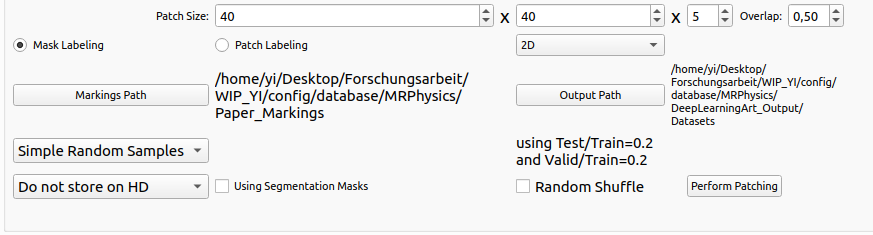
\includegraphics[width=\textwidth]{perform_patching.png}
	\caption[Perform Patching]{Perform Patching}
	\label{fig:perform_patching}
\end{figure}

\subsection{Training neural network}
After you select datasets by either using the current datasets or selecting from path, the network training section on the window will be enabled. You can choose a neural network in the drop down box. If the desired model is not in the list, you can click \textit{add new architecture} at the bottom in the network list to load a prepared architecture from path 'networks'. Then, you can select if you want to use data augmentation and which methods to deploy. Further, you can select batchsize and number of epochs for training neural network. Besides, you can choose the optimizer and number of GPU in the corresponding drop down box. When every options are ready, you can start \textit{Perform Training} neural network. Then an individual network interface will pop up showing all the information in a structured list, including parameters and paths. After the neural network is compiled, it will start training process. After each epoch, there will be two diagrams showing the development of accuracy and loss for both training and validation in the area of \textit{Training Performance}. All the files will be saved, including checkpoints, model in the format of HDF5, model weights, model architecture in the format of PNG, training datasets and training information. 
\begin{figure}[htbp]	
	\centering
	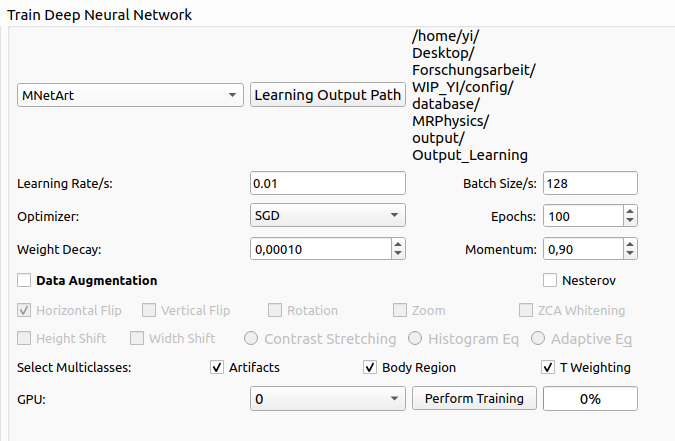
\includegraphics[width=\textwidth]{perform_training.png}
	\caption[Perform Training]{Perform Training}
	\label{fig:perform_training}
\end{figure}
\begin{figure}[htbp]	
	\centering
	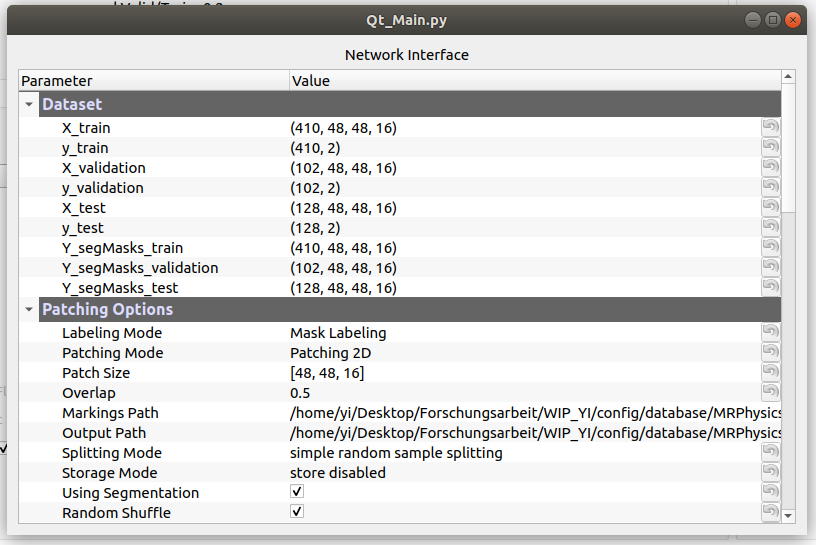
\includegraphics[width=\textwidth]{network_interface.png}
	\caption[Network Interface]{Network Interface}
	\label{fig:network_interface}
\end{figure}

\end{document}
